\chapter{Conclusion and future works}

\section{Conclusion}

Our works began in early September 2024, we choose the problem to tackle with based on our interest and familiar domain. The problem defining phase started with how we can utilize the LLMs to help us with develop a rapidly changing framework with newest guideline. On the other side, we did research about on the background knowledge. We with began with reading surveys about RAG \cite{zhao2024retrievalaugmentedgenerationaigeneratedcontent, gao2023ragllmsurvey} and then dwell in RAG's main components:
\begin{itemize}
	\item Retriever: 
	Begin with how can we represent the data to semantically searchable, the BGE-M3 \cite{chen2024bge} have the exact answer, for our intended language English, multiple searh method from sparse, dense, multiple vectors to hybrid search combine all of them.
	After that we must decide to facilitate the search process, we read about the Knns, and its drawback mainly on the scaling factor, it can't function on a large database. We then decide to choose HNSW \cite{malkov2018hnsw} to mitigate this problem by an acceptable trade off of accuracy with a much more scalable way to search vector.
	\item Generator:
	We started with the Transformer architecture \cite{vaswani2017} laid the foundation for LLMs, which is basically a decoder only transformer, and then choose Qwen \cite{bai2023qwen} to be our model for generate text and code for the system.
\end{itemize}

Later with the suggestion of our supervisor, we decide with serve our approach to the problem in a form of a VSCode extension, we research about related tools going through them based their funtionality retrieval mechanisms, code generation capabilities, integration within development process.


% \begin{figure}[H]
%     \centering
%     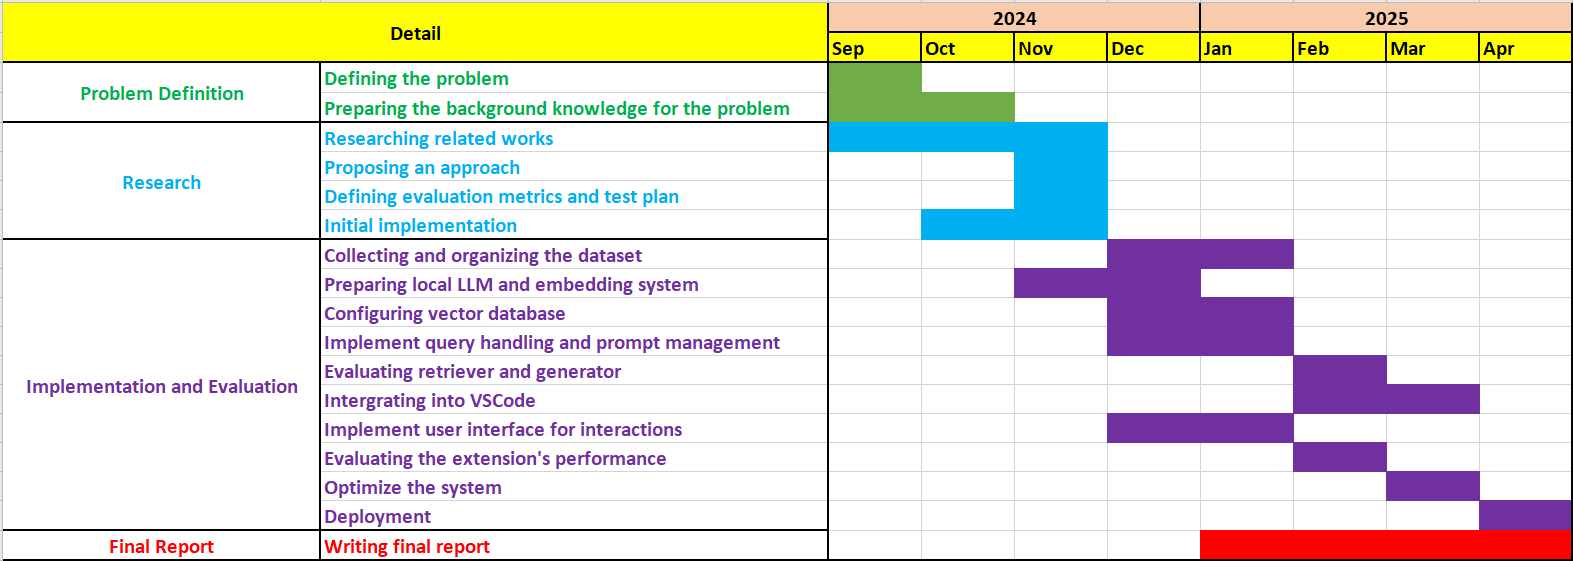
\includegraphics[width=\linewidth]{Images/Conclusion/future_plan_gantt.png}
%     \vspace{0.35cm}
%     \caption{Future plan}
%     \label{fig:future-plan}
% \end{figure}

% \begin{figure}[tbp]
%     \begin{center}
    
%     \begin{ganttchart}[y unit title=0.4cm,
%     y unit chart=0.5cm,
%     x unit=0.7cm,
%     vgrid,hgrid, 
%     % bar/.append style={fill=blue!40, align=left, text width=4cm, text left shift=0.2cm}, % Aligns text left
%     % bar height=0.6,
%     title label anchor/.style={below=-1.6ex},
%     title left shift=.05,
%     title right shift=-.05,
%     title height=1,
%     progress label text={},
%     bar height=0.7,
%     group right shift=0,
%     group top shift=.6,
%     group height=.3]{1}{16}
%     %labels
%     \gantttitle{2024}{8}
%     \gantttitle{2025}{8} \\
%     \gantttitle{Sep}{2} 
%     \gantttitle{Oct}{2} 
%     \gantttitle{Nov}{2} 
%     \gantttitle{Dec}{2} 
%     \gantttitle{Jan}{2} 
%     \gantttitle{Feb}{2} 
%     \gantttitle{Mar}{2} 
%     \gantttitle{Apr}{2} \\
%     %tasks
%     \ganttgroup[progress=100]{Problem Definition}{1}{6} \\
    
%     \ganttbar[progress=100]{Defining the problem}{1}{2}\\
%     \ganttbar[progress=100]{Preparing the background knowledge for the problem}{1}{4}\\

%     \ganttgroup[progress=100]{Research}{1}{9} \\
    
%     \ganttbar[progress=100]{Researching related works}{1}{9}\\
%     \ganttbar[progress=100]{Proposing an approach}{1}{4}\\
%     \ganttbar[progress=100]{Defining evaluation metrics and test plan}{1}{4}\\
    
%     % \ganttbar{first task}{1}{2} \\
%     % \ganttbar{task 2}{3}{8} \\
%     % \ganttbar{task 3}{9}{10} \\
%     % \ganttbar{task 4}{11}{15} \\
%     % \ganttbar[progress=33]{task 5}{20}{22} \\
%     % \ganttbar{task 6}{18}{19} \\
%     % \ganttbar{task 7}{16}{18} \\
%     % \ganttbar[progress=0]{task 8}{21}{24}
    
%     %relations 
%     % \ganttlink{elem0}{elem1} 
%     % \ganttlink{elem0}{elem3} 
%     % \ganttlink{elem1}{elem2} 
%     % \ganttlink{elem3}{elem4} 
%     % \ganttlink{elem1}{elem5} 
%     % \ganttlink{elem3}{elem5} 
%     % \ganttlink{elem2}{elem6} 
%     % \ganttlink{elem3}{elem6} 
%     % \ganttlink{elem5}{elem7} 
%     \end{ganttchart}
%     \end{center}
%     \caption{Gantt Chart}

% \end{figure}

% \begin{ganttchart}{1}{12}
%   \gantttitle{2011}{12} \\
%   \gantttitlelist{1,...,12}{1} \\
%   \ganttgroup{Group 1}{1}{7} \\
%   \ganttbar{Task 1}{1}{2} \\
%   \ganttlinkedbar{Task 2}{3}{7} \ganttnewline
%   \ganttmilestone{Milestone}{7} \ganttnewline
%   \ganttbar{Final Task}{8}{12}
%   \ganttlink{elem2}{elem3}
%   \ganttlink{elem3}{elem4}
% \end{ganttchart}



\section{Upcoming works: January 2025 and beyond}


\begin{enumerate}
	\item \textbf{Preparing local LLM and embedding system (November 2024 -- January 2025):}
	Setup and configure the local LLM and embedding system to handle efficient information retrieval.
	
	\item \textbf{Collecting and organizing the dataset (December 2024 -- February 2025):}
	Data collection and preprocessing efforts will focus on organizing high-quality and relevant datasets.
	
	\item \textbf{Configuring vector database (December 2024 -- February 2025):}
	Establish the vector database to efficiently store and retrieve embeddings for core functionalities.
	
	\item \textbf{Implementing query handling and prompt management (December 2024 -- February 2025):}
	Mechanisms for managing user queries and prompt workflows will be implemented for smooth operations.
	
	\item \textbf{Evaluating retriever and generator (February 2025):}
	Assessment of retrieval and generation components for accuracy, efficiency, and robustness.
	
	\item \textbf{Integrating into VSCode (February -- March 2025):}
	The system will be integrated into the VSCode environment as an extension to improve developer accessibility.
	
	\item \textbf{Implementing user interface for interactions (February -- April 2025):}
	Develop an intuitive and interactive user interface to ensure seamless user experience.
	
	\item \textbf{Evaluating the extension's performance (March 2025):}
	Performance testing of the VSCode extension will focus on usability, responsiveness, and reliability.
	
	\item \textbf{Optimizing the system (March -- May 2025):}
	Optimize the system to enhance efficiency, accuracy, and overall performance.
	
	\item \textbf{Deployment (April -- May 2025):}
	Fully develop, test, and deploy the optimized system for production use.
	
	\item \textbf{Continue writing report (December 2024 -- May 2025):}
	Prepare the final report summarizing the problem definition, research, implementation, evaluation, and findings.
\end{enumerate}

% \hspace{-4cm}
\begin{figure}[tbp]
	% \begin{center}
		\hspace*{-2cm} 
		\begin{ganttchart}[
			y unit title=0.4cm,
			y unit chart=0.6cm,
			x unit=0.6cm,
			vgrid,
			hgrid,
			title label anchor/.style={below=-1.6ex},
			title left shift=.05,
			title right shift=-.05,
			title height=1,
			progress label text={},
			bar height=0.6,
			group right shift=0,
			group top shift=.6,
			group height=.3
			]{1}{18}
			
			% Year and Month Titles
			\gantttitle{2024}{8}
			\gantttitle{2025}{10} \\
			\gantttitle{Sep}{2}
			\gantttitle{Oct}{2}
			\gantttitle{Nov}{2}
			\gantttitle{Dec}{2}
			\gantttitle{Jan}{2}
			\gantttitle{Feb}{2}
			\gantttitle{Mar}{2}
			\gantttitle{Apr}{2} 
			\gantttitle{May}{2} \\
			
			% Problem Definition Group
			\ganttgroup[/pgfgantt/group/.style={},inline=false]{Problem Definition}{1}{7} \\
			\ganttbar[bar/.append style={fill={dkgreen}}]{Defining the problem}{1}{3} \\
			\ganttbar[bar/.append style={fill={dkgreen}}]{Preparing background knowledge}{1}{5} \\
			
			% Research Group
			\ganttgroup[/pgfgantt/group/.style={},inline=false]{Research}{1}{7} \\
			\ganttbar[bar/.append style={fill=cyan}]{Researching related works and tools}{1}{6} \\
			\ganttbar[bar/.append style={fill=cyan}]{Proposing an approach}{4}{6} \\
			\ganttbar[bar/.append style={fill=cyan}]{Defining evaluation metrics and test plan}{5}{7} \\
			\ganttbar[bar/.append style={fill=cyan}]{Initial implementation}{4}{7} \\
			\ganttbar[bar/.append style={fill=cyan}]{Writing report}{3}{7} \\
			% Implementation and Evaluation Group
			\ganttgroup[/pgfgantt/group/.style={},inline=false]{Implementation and evaluation}{5}{18} \\
			\ganttbar[bar/.append style={fill={codepurple}}]{Preparing local LLM and embedding system}{5}{9} \\
			\ganttbar[bar/.append style={fill={codepurple}}]{Collecting and organizing dataset}{7}{11} \\
			\ganttbar[bar/.append style={fill={codepurple}}]{Configuring vector database}{7}{11} \\
			\ganttbar[bar/.append style={fill={codepurple}}]{Implementing query handling and prompt management}{9}{13} \\
			\ganttbar[bar/.append style={fill={codepurple}}]{Evaluating retriever and generator}{11}{13} \\
			\ganttbar[bar/.append style={fill={codepurple}}]{Integrating into VSCode}{11}{15} \\
			\ganttbar[bar/.append style={fill={codepurple}}]{Implementing user interface for interactions}{7}{13} \\
			% \ganttbar[progress=10]{Implement user interface for interactions}{13}{14} \\
			\ganttbar[bar/.append style={fill={codepurple}}]{Evaluating the extension's performance}{13}{16} \\
			\ganttbar[bar/.append style={fill={codepurple}}]{Optimizing the system}{14}{17} \\
			\ganttbar[bar/.append style={fill={codepurple}}]{Deployment}{15}{17} \\
			
			% Final Report Group
			\ganttgroup[/pgfgantt/group/.style={},inline=false]{Final report}{9}{18} \\
			\ganttbar[bar/.append style={fill=red}]{Continue writing report}{9}{17} \\
			
		\end{ganttchart}
		% \end{center}
	\vspace{2mm}
	\caption{Future works.}
\end{figure}
  